%!TEX program = xelatex
\documentclass[UTF8]{ctexart}

% math bracket
%  ()
\newcommand{\brc}[1]{\left({{}#1}\right)}
%  []
\newcommand{\brm}[1]{\left[{{}#1}\right]}
%  ||
\newcommand{\brv}[1]{\left|{{}#1}\right|}
%  {}
\newcommand{\brf}[1]{\left\{{{}#1}\right\}}
%  ||
\newcommand{\brt}[1]{\left\Vert{{}#1}\right\Vert}
%  <>
\newcommand{\brg}[1]{\left<{{}#1}\right>}
%  floor
\newcommand{\floor}[1]{\lfloor{{}#1}\rfloor}
%  ceil
\newcommand{\ceil}[1]{\lceil{{}#1}\rceil}

% font
\newcommand{\fira}[1]{{\firacode {}#1}}

% abbr command
\newcommand{\ds}{\displaystyle}
\newcommand{\pt}{\partial}
\newcommand{\rint}[2]{\Big|^{{}#1}_{{}#2}}
\newcommand{\leg}{\left\lgroup}
\newcommand{\rig}{\right\rgroup}

% math symbol
\newcommand{\de}{\mathrm{d}}
\newcommand{\im}{\mathrm{im}}
\newcommand{\ord}{\mathrm{ord}}
\newcommand{\cov}{\mathrm{Cov}}
\newcommand{\lub}{\mathrm{LUB}}
\newcommand{\glb}{\mathrm{GLB}}
\newcommand{\var}{\mathrm{Var}}
\newcommand{\aut}{\mathrm{Aut}}
\newcommand{\sylow}{\mathrm{Sylow}}
\newcommand{\xhi}{\mathcal{X}}
\newcommand{\po}{\mathcal{P}}
\newcommand{\bi}{\mathrm{b}}
\newcommand{\rfl}{\mathcal{R}}

% algorithmic symbol
\newcommand{\gro}{\mathrm{O}}

\newfontfamily\firacode{Fira Code}
\newfontfamily\mincho{MS Mincho}

% math
\usepackage{ntheorem}
\usepackage{ulem}

\theoremseparator{ }
\newtheorem{dft}{Definition}
\newtheorem{tem}[dft]{Theorem}
\newtheorem{lem}[dft]{Lemma}
\newtheorem{epe}[dft]{Example}
\newtheorem{cor}[dft]{Corollary}

\usepackage{mathrsfs}
\usepackage{amsmath}
\usepackage{amssymb}
\usepackage{cancel}
%\usepackage{amsthm}

% control
\usepackage{ifthen}
\usepackage{intcalc}

% format
\usepackage{indentfirst}
\usepackage{enumerate}
\usepackage{url}
\usepackage{setspace}

\usepackage{xcolor}

\definecolor{ballblue}{rgb}{0.13, 0.67, 0.8}
\definecolor{celestialblue}{rgb}{0.29, 0.59, 0.82}
\definecolor{bananayellow}{rgb}{1.0, 0.88, 0.21}
\definecolor{brilliantlavender}{rgb}{0.96, 0.73, 1.0}
\definecolor{burgundy}{rgb}{0.5, 0.0, 0.13}
\definecolor{cadmiumorange}{rgb}{0.93, 0.53, 0.18}
\definecolor{aqua}{rgb}{0.0, 1.0, 1.0}
\definecolor{auburn}{rgb}{0.43, 0.21, 0.1}
\definecolor{brass}{rgb}{0.71, 0.65, 0.26}
\definecolor{tangerine}{rgb}{0.95, 0.52, 0.0}
\definecolor{portlandorange}{rgb}{1.0, 0.35, 0.21}
\definecolor{mediumred-violet}{rgb}{0.73, 0.2, 0.52}

% listing set
\definecolor{func}{rgb}{0.29, 0.59, 0.82}
\definecolor{ftype}{rgb}{0.95, 0.52, 0.0}
\definecolor{cls}{rgb}{1.0, 0.35, 0.21}
\definecolor{slf}{rgb}{0.73, 0.2, 0.52}
\definecolor{backg}{HTML}{F7F7F7}
\definecolor{str}{HTML}{228B22}
% attestation
\definecolor{atte}{RGB}{178,34,34}

\usepackage{listings}

\lstset{
    backgroundcolor = \color{backg},
    basicstyle = \small,%
    escapeinside = ``,%
    keywordstyle = \color{func},% \underbar,%
    identifierstyle = {},%
    commentstyle = \color{blue},%
    stringstyle = \color{str}\ttfamily,%
    %labelstyle = \tiny,%
    extendedchars = false,%
    linewidth = \textwidth,%
}

\usepackage{geometry}

\geometry{
    left=2.0cm,
    right=2.0cm,
    top=2.5cm,
    bottom=2.5cm
}

\usepackage[
    colorlinks,
    linkcolor=blue,
    anchorcolor=blue,
    citecolor=blue
]{hyperref}

% table
\usepackage{csvsimple}

% graph
\usepackage{tikz}
\usepackage{pgfplots}
\usetikzlibrary{
    quotes,
    angles,
    matrix,
    arrows,
    automata
}


\title{自制操作系统-准备篇}
\author{向阳曦\ 2017211279\ 2017211301}
\date{}

\begin{document}
\setlength{\parindent}{2em}
%\renewcommand{\baselinestretch}{1.5}
\setlength{\baselineskip}{2.5em}
\maketitle
\section{课题硬件环境描述}

\begin{enumerate}[1]
	\item 硬件: TEC-8实验电路
	\begin{enumerate}[1]
		\item 74181ALU等
		\item 可编程逻辑芯片EPM7128
	\end{enumerate}
	\item 软件: Quartus II 9.0
\end{enumerate}

\section{题目分析}
\subsection{实验目标}

\begin{enumerate}[1]
	\item 完成硬连线控制器基础设计
	\item 在原指令的基础上扩指至少三条
	\item 修改PC指针功能
	\item 完成流水硬连线控制器基础设计
	\item 在原指令的基础上扩指至少三条
	\item 修改PC指针功能
\end{enumerate}

\subsection{设计思路}

\begin{enumerate}[1]
	\item 画出硬连线控制器运行流程图
	\item 将硬连线控制器运行流程图翻译成硬连线信号
	\item 将硬连线信号翻译成VHDL多分支程序
\end{enumerate}

\section{团队分工}
向阳曦负责程序指令翻译, 张逸群负责控制台程序。\\
合并一起以后,两人一起完成控制器程序的测试。
\section{设计详解}
\subsection{硬连线控制器}
\subsubsection{设计硬连线控制器运行流程图}

\begin{figure}[!h]
    \centering
    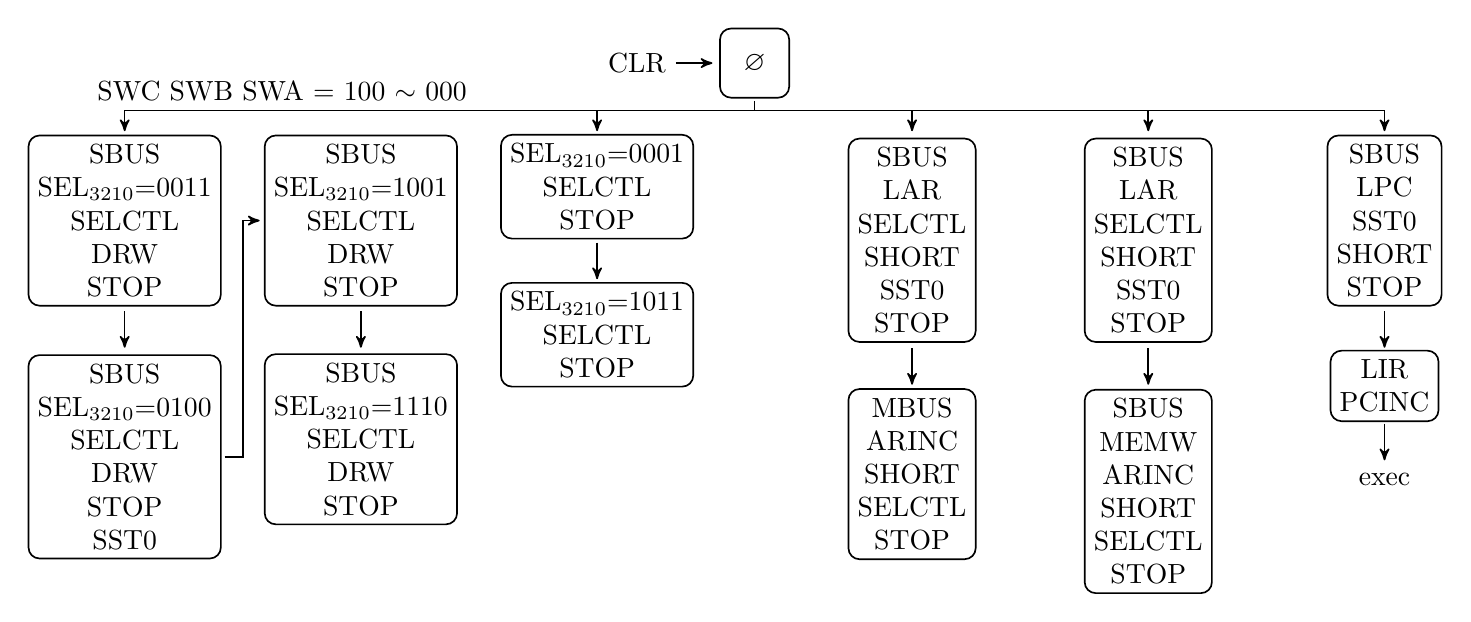
\begin{tikzpicture}[->,>=stealth',shorten >=1pt,auto,node distance=2.8cm,semithick]
    \tikzstyle{every state}=[shape=rectangle, rounded corners]
	\node[left] (clr) at (-1, 0) {CLR}; 
	\draw [->] (-1, 0) -- (-0.5,0);
	\node[state] (A) at (0, 0) {$\varnothing$};
	\node[state, align=center] (readra) at ( -8, -2) {SBUS\\ $\text{SEL}_{3210}$=0011\\ SELCTL\\ DRW\\ STOP};
	
	\node[state, align=center] (readrb) at ( -5, -2) {SBUS\\ $\text{SEL}_{3210}$=1001\\ SELCTL\\ DRW\\ STOP};

	\node[state, align=center] (readrc) at ( -8, -5) {SBUS\\ $\text{SEL}_{3210}$=0100\\ SELCTL\\ DRW\\ STOP\\ SST0};

	\node[state, align=center] (readrd) at ( -5, -4.777 ) {SBUS\\ $\text{SEL}_{3210}$=1110\\ SELCTL\\ DRW\\ STOP};
	
	\node[state, align=center] (readrd) at ( -2, -1.57 ) {$\text{SEL}_{3210}$=0001\\ SELCTL\\ STOP};
	\node[state, align=center] (readrd) at ( -2, -3.45 ) {$\text{SEL}_{3210}$=1011\\ SELCTL\\ STOP};

	\node[state, align=center] (readrd) at ( 2, -2.25 ) {SBUS\\ LAR\\ SELCTL\\ SHORT \\ SST0\\ STOP};
	\node[state, align=center] (readrd) at ( 2, -5.22 ) {MBUS\\ ARINC\\ SHORT\\ SELCTL\\ STOP};

	\node[state, align=center] (readrd) at ( 5, -2.25 ) {SBUS\\ LAR\\ SELCTL\\ SHORT \\ SST0\\ STOP};
	\node[state, align=center] (readrd) at ( 5, -5.44 ) {SBUS\\ MEMW\\ ARINC\\ SHORT\\ SELCTL\\ STOP};

	\node[state, align=center] (readrd) at ( 8, -2 ) {SBUS\\ LPC\\ SST0\\ SHORT\\ STOP};
	\node[state, align=center] (readrd) at ( 8, -4.10 ) {LIR \\ PCINC};
	%\path (A) edge[bend left] (B)
	\draw [->] (0, -0.48) -- (0, -0.6) -- (-8, -0.6) -- (-8, -0.9);
	\draw [->] (-8, -3.15) -- (-8, -3.65);
	\draw [->] (-6.73, -5) -- (-6.5, -5) -- (-6.5, -2) -- (-6.25, -2);
	\draw [->] (-5, -3.15) -- (-5, -3.65);

	\draw [->] (-2, -0.6) -- (-2, -0.9);
	\draw [->] (-2, -2.28) -- (-2, -2.78);

	\draw [->] (0, -0.6) -- (2, -0.6)-- (2, -0.9);
	\draw [->] (2, -3.62) -- (2, -4.12);
	
	\draw [->] (2, -0.6) -- (5, -0.6) -- (5, -0.9);
	\draw [->] (5, -3.62) -- (5, -4.12);
	
	\draw [->] (5, -0.6) -- (8, -0.6) -- (8, -0.9);

	\draw [->] (8, -3.15) -- (8, -3.65);
	\draw [->] (8, -4.58) -- (8, -5.08) node [below] {exec};

	\node [above] at (-6, -0.6) {SWC SWB SWA = 100 $\sim$ 000};
    \end{tikzpicture}
\end{figure}
其中CLR表示转移到$\varnothing$.任意没有出边的状态也都转移到$\varnothing$,任意时刻传入CLR信号也都转移到$\varnothing$.
\newpage
\begin{figure}[!h]
    \centering
    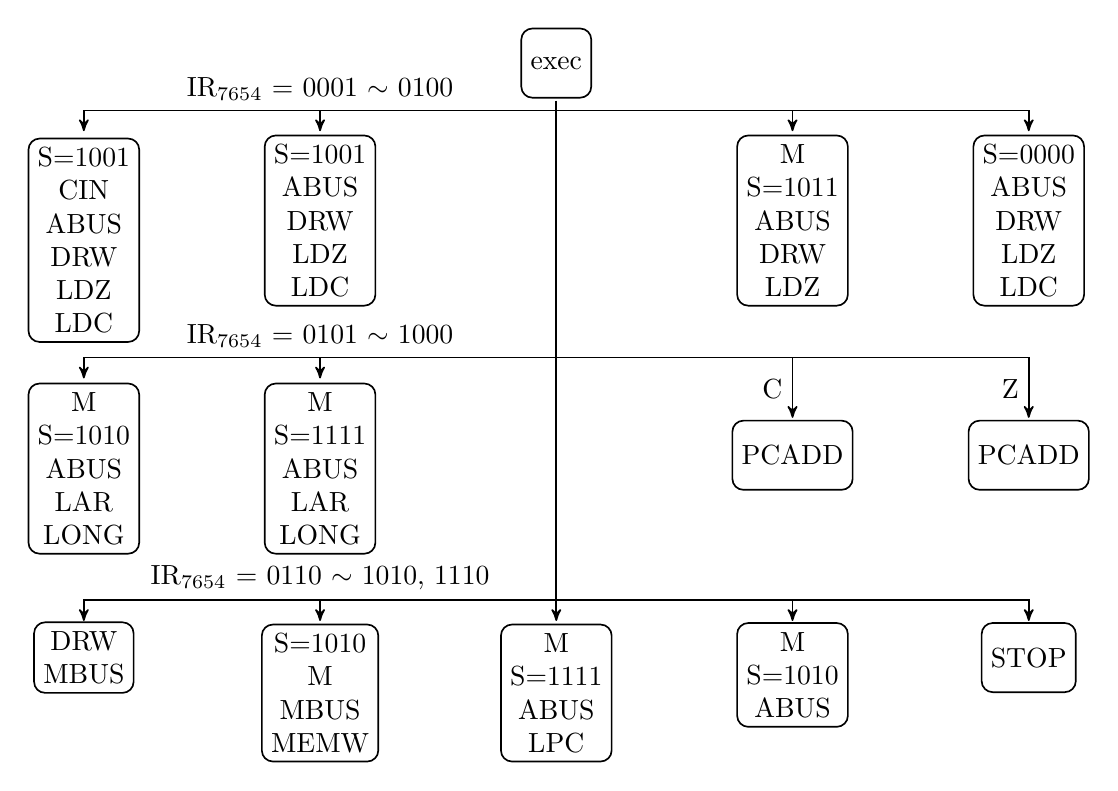
\begin{tikzpicture}[->,>=stealth',shorten >=1pt,auto,node distance=2.8cm,semithick]
    \tikzstyle{every state}=[shape=rectangle, rounded corners]
	\node [state] (A) at (0, 0) {exec};
	\node [state, align = center] at (-6, -2.25) {S=1001\\ CIN \\ ABUS\\ DRW\\ LDZ\\ LDC};
	
	\node [state, align = center] at (-3, -2) {S=1001 \\ ABUS\\ DRW\\ LDZ\\ LDC};
	
	\node [state, align = center] at (3, -2) {M\\ S=1011 \\ ABUS\\ DRW\\ LDZ};

	\node [state, align = center] at (6, -2) { S=0000 \\ ABUS\\ DRW\\ LDZ\\ LDC};

	\node [state, align = center] at (-6, -5.15) { M\\ S=1010 \\ ABUS\\ LAR\\ LONG};
	
	\node [state, align = center] at (-6, -7.55) {DRW\\ MBUS};

	\node [state, align = center] at (-3, -5.15) { M\\ S=1111 \\ ABUS\\ LAR\\ LONG};

	\node [state, align = center] at (-3, -8) {S=1010\\ M\\ MBUS\\ MEMW};
	
	\node [state, align = center] at (3, -4.98) {PCADD};

	\node [state, align = center] at (6, -4.98) {PCADD};
	
	\node [state, align = center] at (0, -8) {M\\S=1111\\ ABUS\\ LPC};

	\node [state, align = center] at (3, -7.77) {M\\S=1010\\ ABUS};
	
	\node [state, align = center] at (6, -7.55) {STOP};
	
	\draw [->] (0, -0.48) -- (0, -0.6) -- (-6, -0.6) -- (-6, -0.9);
	\draw [->] (-3, -0.6) -- (-3, -0.9);
	\draw [->] (0, -0.48) -- (0, -0.6) -- (6, -0.6) -- (6, -0.9);
	\draw [->] (3, -0.6) -- (3, -0.9);

	\draw [->] (0, -0.6) -- (0, -3.74) -- (-6, -3.74) -- (-6, -4.04);
	\draw [->] (-3, -3.74) -- (-3, -4.04);
	\draw [->] (0, -3.74) -- (6, -3.74) -- node [left]{Z} (6, -4.54);
	\draw [->] (3, -3.74) -- node [left]{C} (3, -4.54);

	\draw [->] (0, -3.74) -- (0, -6.82) -- (-6, -6.82) -- (-6, -7.12);
	\draw [->] (-3, -6.82) -- (-3, -7.12);
	\draw [->] (0, -6.82) -- (0, -7.12);
	\draw [->] (0, -6.82) -- (6, -6.82) -- (6, -7.12);
	\draw [->] (3, -6.82) -- (3, -7.12);
	\node [above] at (-3, -0.6) {$\text{IR}_{7654}$ = 0001 $\sim$ 0100};
	\node [above] at (-3, -3.74) {$\text{IR}_{7654}$ = 0101 $\sim$ 1000};
	\node [above] at (-3, -6.82) {$\text{IR}_{7654}$ = 0110 $\sim$ 1010, 1110};
	\end{tikzpicture}
\end{figure}
上图显示了从左到右,从上到下依次为ADD, SUB, AND, INC, LD, ST, JC, JZ, JMP, OUT, STP的所有指令.\\
需要注意的是,如果某条指令包含SHORT,那么它是一个单拍指令,
如果某条指令包含LONG,那么它的下一拍还属于该指令, 计三拍.
\subsubsection{翻译成硬连线信号}
\noindent SBUS $\leftarrow$
\begin{enumerate}[\indent\indent]
	\item $(\text{W1} + \text{W2}) \cdot \text{SWC} \cdot \overline{\text{SWB}} \cdot \overline{\text{SWA}}$+
	\item $\text{W1} \cdot \overline{\text{SWC}} \cdot \text{SWB} \cdot \overline{\text{SWA}} \cdot \overline {\text{ST0}}$+
	\item $\text{W1} \cdot \overline{\text{SWC}} \cdot\overline{\text{SWB}}\cdot  \text{SWA}$+
​	\item $\text{W1} \cdot \overline{\text{SWC}} \cdot\overline{\text{SWB}}\cdot \overline{\text{SWA}}\cdot \overline{\text{ST0}} $
\end{enumerate}
MBUS $\leftarrow$
\begin{enumerate}[\indent\indent]
	\item $\text{W1} \cdot \overline{\text{SWC}} \cdot \text{SWB} \cdot \overline{\text{SWA}} \cdot \text{ST0}$+
	\item $\text{W3} \cdot \overline{\text{IR7}} \cdot \text{IR6} \cdot \overline{\text{IR5}} \cdot \text{IR4} \cdot \overline{\text{SWC}} \cdot\overline{\text{SWB}}\cdot \overline{\text{SWA}}$
\end{enumerate}
ABUS $\leftarrow$
\begin{enumerate}[\indent\indent]
	\item $\overline{\text{SWC}} \cdot\overline{\text{SWB}}\cdot \overline{\text{SWA}} \cdot \overline{\text{IR7}} \cdot \overline{\text{IR6}} \cdot \overline{\text{IR5}} \cdot \text{IR4} \cdot \text{W2}$+
	\item $\overline{\text{SWC}} \cdot\overline{\text{SWB}}\cdot \overline{\text{SWA}} \cdot \overline{\text{IR7}} \cdot \overline{\text{IR6}} \cdot \text{IR5} \cdot \overline{\text{IR4}} \cdot \text{W2}$+
	\item $\overline{\text{SWC}} \cdot\overline{\text{SWB}}\cdot \overline{\text{SWA}} \cdot \overline{\text{IR7}} \cdot \overline{\text{IR6}} \cdot \text{IR5} \cdot \text{IR4} \cdot \text{W2}$+
	\item $\overline{\text{SWC}} \cdot\overline{\text{SWB}}\cdot \overline{\text{SWA}} \cdot \overline{\text{IR7}} \cdot \text{IR6} \cdot \overline{\text{IR5}} \cdot \overline{\text{IR4}} \cdot \text{W2}$+
	\item $\overline{\text{SWC}} \cdot\overline{\text{SWB}}\cdot \overline{\text{SWA}} \cdot \overline{\text{IR7}} \cdot \text{IR6} \cdot \overline{\text{IR5}} \cdot \text{IR4} \cdot \text{W2}$+
	\item $\overline{\text{SWC}} \cdot\overline{\text{SWB}}\cdot \overline{\text{SWA}} \cdot \overline{\text{IR7}} \cdot \text{IR6} \cdot \text{IR5} \cdot \overline{\text{IR4}} \cdot (\text{W2} + \text{W3})$+
	\item $\overline{\text{SWC}} \cdot\overline{\text{SWB}}\cdot \overline{\text{SWA}} \cdot \text{IR7} \cdot \overline{\text{IR6}} \cdot \overline{\text{IR5}} \cdot \text{IR4} \cdot \text{W2}$+
	\item $\overline{\text{SWC}} \cdot\overline{\text{SWB}}\cdot \overline{\text{SWA}} \cdot \text{IR7} \cdot \overline{\text{IR6}} \cdot \text{IR5} \cdot \overline{\text{IR4}} \cdot \text{W2}$
\end{enumerate}
LAR $\leftarrow$
\begin{enumerate}[\indent\indent]
	\item $\text{W1} \cdot \overline{\text{SWC}} \cdot \text{SWB} \cdot \overline{\text{SWA}} \cdot \overline{\text{ST0}}$+
	\item $\text{W1} \cdot \overline{\text{SWC}} \cdot \overline{\text{SWB}} \cdot \text{SWA} \cdot \overline{\text{ST0}}$+
	\item $\overline{\text{SWC}} \cdot\overline{\text{SWB}}\cdot \overline{\text{SWA}}+ \cdot \overline{\text{IR7}} \cdot \text{IR6} \cdot \overline{\text{IR5}} \cdot \text{IR4} \cdot \text{W2}$+
	\item $\overline{\text{SWC}} \cdot\overline{\text{SWB}}\cdot \overline{\text{SWA}}+ \cdot \overline{\text{IR7}} \cdot \text{IR6} \cdot \text{IR5} \cdot \overline{\text{IR4}} \cdot \text{W2}$
\end{enumerate}
SST0 $\leftarrow$
\begin{enumerate}[\indent\indent]
	\item $\text{W1} \cdot \overline{\text{SWC}} \cdot \text{SWB} \cdot \overline{\text{SWA}} \cdot \overline{\text{ST0}}$+
	\item $\text{W2} \cdot \text{SWC} \cdot \overline{\text{SWB}} \cdot \overline{\text{SWA}} \cdot \overline{\text{ST0}}$+
	\item $\text{W1} \cdot \overline{\text{SWC}} \cdot \overline{\text{SWB}} \cdot \text{SWA} \cdot \overline{\text{ST0}}$+
	\item $\text{W1} \cdot \overline{\text{SWC}} \cdot \overline{\text{SWB}} \cdot \overline{\text{SWA}} \cdot \overline{\text{ST0}}$
\end{enumerate}
SHORT $\leftarrow$
\begin{enumerate}[\indent\indent]
	\item $\text{W1} \cdot \overline{\text{SWC}} \cdot \text{SWB} \cdot \overline{\text{SWA}}$+
	\item $\text{W1} \cdot \overline{\text{SWC}} \cdot \overline{\text{SWB}} \cdot \text{SWA}$+
	\item $\text{W1} \cdot \overline{\text{SWC}} \cdot \overline{\text{SWB}} \cdot \overline{\text{SWA}} \cdot \overline{ST0}$
\end{enumerate}
ARINC $\leftarrow$
\begin{enumerate}[\indent\indent]
	\item $\text{W1} \cdot \overline{\text{SWC}} \cdot \text{SWB} \cdot \overline{\text{SWA}} \cdot \text{ST0}$+
	\item $\text{W1} \cdot \overline{\text{SWC}} \cdot \overline{\text{SWB}} \cdot \text{SWA} \cdot \text{ST0}$
\end{enumerate}
MEMW $\leftarrow$
\begin{enumerate}[\indent\indent]
	\item $\text{W1} \cdot \overline{\text{SWC}} \cdot \overline{\text{SWB}} \cdot \text{SWA} \cdot \text{ST0}$+
	\item $\overline{\text{SWC}} \cdot\overline{\text{SWB}}\cdot \overline{\text{SWA}} \cdot \overline{\text{IR7}} \cdot \text{IR6} \cdot \text{IR5} \cdot \overline{\text{IR4}} \cdot \text{W3}$
\end{enumerate}
LIR $\leftarrow$
\begin{enumerate}[\indent\indent]
	\item $\overline{\text{SWC}} \cdot\overline{\text{SWB}}\cdot \overline{\text{SWA}} \cdot \text{ST0} \cdot \text{W1}$
\end{enumerate}
CIN $\leftarrow$
\begin{enumerate}[\indent\indent]
	\item $\overline{\text{SWC}} \cdot\overline{\text{SWB}}\cdot \overline{\text{SWA}} \cdot \overline{\text{IR7}} \cdot \overline{\text{IR6}} \cdot \overline{\text{IR5}} \cdot \overline{\text{IR4}} \cdot \text{W2}$
\end{enumerate}
M $\leftarrow$
\begin{enumerate}[\indent\indent]
	\item $\overline{\text{SWC}} \cdot\overline{\text{SWB}}\cdot \overline{\text{SWA}} \cdot \overline{\text{IR7}} \cdot \overline{\text{IR6}} \cdot \text{IR5} \cdot \text{IR4} \cdot \text{W2}$+
	\item $\overline{\text{SWC}} \cdot\overline{\text{SWB}}\cdot \overline{\text{SWA}} \cdot \overline{\text{IR7}} \cdot \text{IR6} \cdot \overline{\text{IR5}} \cdot \text{IR4} \cdot \text{W2}$+
	\item $\overline{\text{SWC}} \cdot\overline{\text{SWB}}\cdot \overline{\text{SWA}} \cdot \overline{\text{IR7}} \cdot \text{IR6} \cdot \text{IR5} \cdot \overline{\text{IR4}} \cdot (\text{W2} + \text{W3})$+
	\item $\overline{\text{SWC}} \cdot\overline{\text{SWB}}\cdot \overline{\text{SWA}} \cdot \text{IR7} \cdot \overline{\text{IR6}} \cdot \overline{\text{IR5}} \cdot \text{IR4} \cdot \text{W2}$+
	\item $\overline{\text{SWC}} \cdot\overline{\text{SWB}}\cdot \overline{\text{SWA}} \cdot \text{IR7} \cdot \overline{\text{IR6}} \cdot \text{IR5} \cdot \overline{\text{IR4}} \cdot \text{W2}$
\end{enumerate}
SEL0$\leftarrow$
\begin{enumerate}[\indent\indent]
	\item$\text{SWC}\cdot\overline{\text{SWB}}\cdot\overline{\text{SWA}}\cdot\text{W1}$
\end{enumerate}
SEL1$\leftarrow$
\begin{enumerate}[\indent\indent]
	\item$\text{SWC}\cdot\overline{\text{SWB}}\cdot\overline{\text{SWA}}\cdot\text{W2}\cdot\text{ST0}$
	\item$\text{SWC}\cdot\overline{\text{SWB}}\cdot\overline{\text{SWA}}\cdot\text{W1}\cdot\overline{\text{ST0}}$
\end{enumerate}
SEL2$\leftarrow$
\begin{enumerate}[\indent\indent]
	\item$\text{SWC}\cdot\overline{\text{SWB}}\cdot\overline{\text{SWA}}\cdot\text{W2}$
\end{enumerate}
SEL3$\leftarrow$
\begin{enumerate}[\indent\indent]
	\item$\text{SWC}\cdot\overline{\text{SWB}}\cdot\overline{\text{SWA}}\cdot\text{W1}\cdot\text{ST0}$+
	\item$\text{SWC}\cdot\overline{\text{SWB}}\cdot\overline{\text{SWA}}\cdot\text{W2}\cdot\overline{\text{ST0}}$
\end{enumerate}		
STOP$\leftarrow$
\begin{enumerate}[\indent\indent]
	\item$\text{SWA}+\text{SWB}+\text{SWC}$+
	\item$\overline{\text{SWC}}\cdot\overline{\text{SWB}}\cdot\overline{\text{SWA}}\cdot {\text{IR7}} \cdot {\text{IR6}}\cdot {\text{IR5}}\cdot \overline{\text{IR4}} \cdot \text{ST0}\cdot \text{W2}$
\end{enumerate}
SELCTL$\leftarrow$
\begin{enumerate}[\indent\indent]
	\item$\text{SWA}+\text{SWB}+\text{SWC}$
\end{enumerate}
DRW$\leftarrow$
\begin{enumerate}[\indent\indent]
	\item$\text{SWC}\cdot\overline{\text{SWB}}\cdot\overline{\text{SWA}}$+
	\item$\overline{\text{SWC}}\cdot\overline{\text{SWB}}\cdot\overline{\text{SWA}}\cdot\text{ST0}\cdot\overline{\text{IR7}}\cdot\overline{\text{IR6}}\cdot\overline{\text{IR5}}\cdot\text{IR4}\cdot\text{W2}$+
	\item$\overline{\text{SWC}}\cdot\overline{\text{SWB}}\cdot\overline{\text{SWA}}\cdot\text{ST0}\cdot\overline{\text{IR7}}\cdot\overline{\text{IR6}}\cdot{\text{IR5}}\cdot\overline{\text{IR4}}\cdot\text{W2}$+
	\item$\overline{\text{SWC}}\cdot\overline{\text{SWB}}\cdot\overline{\text{SWA}}\cdot\text{ST0}\cdot\overline{\text{IR7}}\cdot\overline{\text{IR6}}\cdot\text{IR5}\cdot\text{IR4}\cdot\text{W2}$+
	\item$\overline{\text{SWC}}\cdot\overline{\text{SWB}}\cdot\overline{\text{SWA}}\cdot\text{ST0}\cdot\overline{\text{IR7}}\cdot{\text{IR6}}\cdot\overline{\text{IR5}}\cdot\overline{\text{IR4}}\cdot\text{W2}$+
	\item$\overline{\text{SWC}}\cdot\overline{\text{SWB}}\cdot\overline{\text{SWA}}\cdot\text{ST0}\cdot\overline{\text{IR7}}\cdot{\text{IR6}}\cdot\overline{\text{IR5}}\cdot{\text{IR4}}\cdot\text{W3}$
\end{enumerate}
PCADD$\leftarrow$
\begin{enumerate}[\indent\indent]
	\item$\overline{\text{SWC}}\cdot\overline{\text{SWB}}\cdot\overline{\text{SWA}}\cdot\text{ST0}\cdot\overline{\text{IR7}}\cdot{\text{IR6}}\cdot{\text{IR5}}\cdot{\text{IR4}}\cdot\text{C}\cdot\text{W2}$+
	\item$\overline{\text{SWC}}\cdot\overline{\text{SWB}}\cdot\overline{\text{SWA}}\cdot\text{ST0}\cdot{\text{IR7}}\cdot\overline{\text{IR6}}\cdot\overline{\text{IR5}}\cdot\overline{\text{IR4}}\cdot\text{Z}\cdot\text{W2}$
\end{enumerate}
PCINC$\leftarrow$
\begin{enumerate}[\indent\indent]
	\item$\overline{\text{SWC}}\cdot\overline{\text{SWB}}\cdot\overline{\text{SWA}}\cdot\text{ST0}\cdot\text{W1}$
\end{enumerate}
LPC$\leftarrow$
\begin{enumerate}[\indent\indent]
	\item$\overline{\text{SWC}}\cdot\overline{\text{SWB}}\cdot\overline{\text{SWA}}\cdot\overline{\text{ST0}}\cdot\text{W2}$
\end{enumerate}
LONG$\leftarrow$
\begin{enumerate}[\indent\indent]
	\item$\overline{\text{SWC}}\cdot\overline{\text{SWB}}\cdot\overline{\text{SWA}}\cdot\text{W2}\cdot\overline{\text{IR7}}\cdot{\text{IR6}}\cdot\overline{\text{IR5}}\cdot{\text{IR4}}$+
	\item$\overline{\text{SWC}}\cdot\overline{\text{SWB}}\cdot\overline{\text{SWA}}\cdot\text{W2}\cdot\overline{\text{IR7}}\cdot{\text{IR6}}\cdot{\text{IR5}}\cdot\overline{\text{IR4}}$
\end{enumerate}
LDC$\leftarrow$
\begin{enumerate}[\indent\indent]
	\item$\overline{\text{SWC}}\cdot\overline{\text{SWB}}\cdot\overline{\text{SWA}}\cdot\text{ST0}\cdot\overline{\text{IR7}}\cdot\overline{\text{IR6}}\cdot\overline{\text{IR5}}\cdot\text{IR4}\cdot\text{W2}$+
	\item$\overline{\text{SWC}}\cdot\overline{\text{SWB}}\cdot\overline{\text{SWA}}\cdot\text{ST0}\cdot\overline{\text{IR7}}\cdot\overline{\text{IR6}}\cdot{\text{IR5}}\cdot\overline{\text{IR4}}\cdot\text{W2}$+
	\item$\overline{\text{SWC}}\cdot\overline{\text{SWB}}\cdot\overline{\text{SWA}}\cdot\text{ST0}\cdot\overline{\text{IR7}}\cdot\overline{\text{IR6}}\cdot\text{IR5}\cdot\text{IR4}\cdot\text{W2}$+
	\item$\overline{\text{SWC}}\cdot\overline{\text{SWB}}\cdot\overline{\text{SWA}}\cdot\text{ST0}\cdot\overline{\text{IR7}}\cdot{\text{IR6}}\cdot\overline{\text{IR5}}\cdot\overline{\text{IR4}}\cdot\text{W2}$
\end{enumerate}
LDZ$\leftarrow$
\begin{enumerate}[\indent\indent]
	\item$\overline{\text{SWC}}\cdot\overline{\text{SWB}}\cdot\overline{\text{SWA}}\cdot\text{ST0}\cdot\overline{\text{IR7}}\cdot\overline{\text{IR6}}\cdot\overline{\text{IR5}}\cdot\text{IR4}\cdot\text{W2}$+
	\item$\overline{\text{SWC}}\cdot\overline{\text{SWB}}\cdot\overline{\text{SWA}}\cdot\text{ST0}\cdot\overline{\text{IR7}}\cdot\overline{\text{IR6}}\cdot{\text{IR5}}\cdot\overline{\text{IR4}}\cdot\text{W2}$+
	\item$\overline{\text{SWC}}\cdot\overline{\text{SWB}}\cdot\overline{\text{SWA}}\cdot\text{ST0}\cdot\overline{\text{IR7}}\cdot\overline{\text{IR6}}\cdot\text{IR5}\cdot\text{IR4}\cdot\text{W2}$+
	\item$\overline{\text{SWC}}\cdot\overline{\text{SWB}}\cdot\overline{\text{SWA}}\cdot\text{ST0}\cdot\overline{\text{IR7}}\cdot{\text{IR6}}\cdot\overline{\text{IR5}}\cdot\overline{\text{IR4}}\cdot\text{W2}$
\end{enumerate}

\subsubsection{翻译成多分支程序}
观察硬连线信号,事实上如果写成VHDL语句,我们可以将$SWCBA$信号合并.然后再在$\overline{SWC}\cdot \overline{SWB}\cdot \overline{SWA}$分支上将$\text{IR}_{7654}$合并.用两个大switch语句完成逻辑分类.

{\firacode
\begin{lstlisting}[language={VHDL}]
library IEEE;
use IEEE.std_logic_1164.all;
use IEEE.std_logic_unsigned.all;
entity CPU is
	port (
		CLR,C,Z,T3,W1,W2,W3: in std_logic;
		IRH:in std_logic_vector(3 downto 0);
		SWCBA:in std_logic_vector(2 downto 0);
		SELCTL,ABUS,M,SEL1,SEL0,SEL2,SEL3,DRW,SBUS,LIR,MBUS,MEMW,LAR,ARINC,LPC,
		PCINC,PCADD,CIN,LONG,SHORT,STOP,LDC,LDZ: out std_logic;
		S:out std_logic_vector(3 downto 0);
		CP1,CP2,CP3:out std_logic;	
		QD:in std_logic	
	);
end CPU;

architecture arc of CPU is
signal ST0,ST0_1,ST0_2,STOP_1,STOP_2: std_logic;
begin
	CP1 <= '1';
	CP2 <= '1';
	CP3 <= QD;
	
	with SWCBA select
		STOP <= '0'						when "000",
				STOP_1 or STOP_2 		when others;
	ST0 <= ST0_1;

	process (CLR, T3)
	begin
		-- 任何时候按下CLR, 都会返回
		if (CLR = '0') then
			ST0_1	<= '0';
			STOP_1	<= '1';
		-- 如果到节拍电位T3下降沿,ST0_1 |= ST0_2
		elsif (T3'event and T3 = '0') then
			if (ST0_2 = '1') then
				ST0_1 <= '1';
			end if;
		end if;
	end process;
	
	process (SWCBA, IRH, W1, W2, W3, ST0, C, Z)
	begin	
		-- 初始化 和 状态参数
		SHORT <= '0';
		LONG <= '0';
		-- 设置STOP
		STOP_2 <= '1';
		-- 设置ST0标志
		ST0_2 <= '0';
		-- ALU
		ABUS <= '0';
		M <= '0';
		CIN <= '0';
		S <= "0000";
		ARINC <= '0';
		-- 保存Z标志
		LDZ <= '0';
		-- 保存C标志
		LDC <= '0';		
		SBUS <= '0';
		MBUS <= '0';
		-- 控制台操作标志
		SELCTL <= '0';
		-- RD1~RD0
		SEL3 <= '0';
		SEL2 <= '0';
		-- RS1~RS0
		SEL1 <= '0';
		SEL0 <= '0';
		-- 送指令寄存器标志
		LIR <= '0';
		-- 送地址寄存器标志
		LAR <= '0';
		-- 送程序计数器标志
		LPC <= '0';
		-- (~R)/W
		MEMW <= '0';
		DRW <= '0';
		-- 程序计数器自增标志
		PCINC <= '0';		
		-- 程序计数器增量标志
		PCADD <= '0';
		case SWCBA is
			when "000" =>  --执行程序
				case ST0 is
					when '0' =>
						-- load pc
						LPC <= W1;
						SBUS <= W1;
						ST0_2 <= W1;
						SHORT <= W1;
						STOP_2 <= '0';
					when '1' =>
						if(W1='1')then
							LIR<=W1;
							PCINC<=W1;
						else                        
					case IRH is 
						when "0001" =>  --ADD 														
							-- ABUS = W2
							ABUS <= W2;
							CIN <= W2;
							-- 选择加法
							-- 选择算术运算, M已经被初始化为0
							S <= "1001";
							-- 加法操作
							DRW <= W2;
							LDZ <= W2;
							LDC <= W2;
						when "0010" =>  -- SUB													
							-- 选择算术运算, 选择减法
							-- M已经被初始化为0
							S <= "0110";
							-- 减法操作
							ABUS <= W2;
							DRW <= W2;
							LDZ <= W2;
							LDC <= W2;
						when "0011" =>  -- AND								
							-- 选择逻辑运算, 与运算
							M <= W2;
							S <= "1011";
							ABUS <= W2;
							DRW <= W2;
							LDZ <= W2;
						when "0100" => -- INC								
							-- 选择算术运算, 与运算
							-- M已经被初始化为0
							S <= "0000";
							ABUS <= W2;
							DRW <= W2;
							LDZ <= W2;
							LDC <= W2;
						when "0101" =>  -- LD
							-- 选择算术运算,传送B(保留原值)
							M <= W2;
							S <= "1010";
							ABUS <= W2;
							LONG<=W2;
							LAR <= W2;
							MBUS <= W3;
							DRW <= W3;
						when "0110" =>  -- ST
							LONG<=W2;
							-- 设定...
							M <= W2 or W3;
							if(W2='1')then
								S<="1111";
							else
								S<="1010";
							end if;
							ABUS <= W2 or W3;
							LAR <= W2;
							MEMW <= W3;							
						when "0111" =>  -- JC
							PCADD <= C and W2;
						when "1000" =>  -- JZ
							PCADD <= Z and W2;
						when "1001" =>  -- JMP
							-- 设定算术运算
							M <= W2;
							S <= "1111";
							ABUS <= W2;
							LPC <= W2;
						when "1010" =>  -- OUT
							-- 设定算术运算
							M <= W2;
							S <= "1010";
							ABUS <= W2;
						when "1011" =>  -- SSP  
							SEL3<='1';
							LONG<=W2;
							M <= W2 or W3;
							if (W2 = '1') then
								S <= "1000";
							elsif (W3 = '1') then
								S <= "1010";
							end if;
							ABUS <= W2 or W3;
							LAR <= W2;
							MEMW <= W3;
						when "1100" =>  -- PUSH
							--PUSH无法自减
							M <= W2 or W3;
							if (W2 = '1') then
								S <= "1111";
							elsif (W3 = '1') then
								S <= "1010";
							end if;
							ABUS <=W2 or W3;
							LAR <= W2;
							MEMW <= W3;
							LONG <= W2;
						when "1101" =>  -- MOV B->A								
							-- 选择逻辑运算, MOV 运算
							M <= W2;
							S <= "1010";
							ABUS <= W2;
							DRW <= W2;
							LDZ <= W2;
						when "1110" =>  -- STP
							STOP_2 <= W2;								
						when "1111" =>  -- LSP
							LONG<=W2;
							M <= W2;
							S <= "1000";
							ABUS <= W2;
							LAR <= W2;
							MBUS <= W3;
							DRW <= W3;		
						when others =>  -- 公操作
					end case;
						end if;
					when others =>
							-- 不可能到这吧?
				end case;
			when "001" =>
			--	SEL0<=ST0;
				-- SBUS = (ST0=0 or ST0=1) and W1 
				SBUS <= W1;
				-- STOP = (ST0=0 or ST0=1) and W1
				STOP_2 <= W1;
				-- SHORT = (ST0=0 or ST0=1) and W1
				SHORT <= W1;
				-- SELCTL = (ST0=0 or ST0=1) and W1
				SELCTL <= W1;
				-- LAR = (ST0=0) and W1
				LAR <= W1 and (not ST0);
				-- LAR = (ST0=1) and W1
				ARINC <= W1 and ST0;
				-- MEMW = (ST0=1) and W1
				MEMW <= W1 and ST0;
				ST0_2 <= W1;
			when "010" =>
				-- SHORT = (ST0=0 or ST0=1) and W1
				SHORT<=W1;
				-- SELCTL = (ST0=0 or ST0=1) and W1
				SELCTL <= W1;
				-- STOP = (ST0=0 or ST0=1) and W1
				STOP_2<=W1;
				-- SBUS = (ST0=0) and W1
				SBUS<=W1 and (not ST0);
				-- LAR = (ST0=0) and W1
				LAR<=W1 and (not ST0);
				-- MBUS = (ST0=1) and W1
				MBUS<=W1 and ST0;
				-- ARINC = (ST0=1) and W1
				ARINC<=W1 and ST0;
				ST0_2<=W1;
			when "011" =>
				-- SELCTL = W1 or W2
				SELCTL <= '1';
				-- STOP = W1 or W2
				STOP_2 <= W1 or W2;
				-- SEL0 = W1 or W2
				SEL0<=W1 or W2;
				-- SEL1 = W2
				SEL1<=W2;
				-- SEL2 = 0
				-- SEL3 = W2
				SEL3<=W2;
			when "100" =>
				-- SELCTL = (ST0=0 or ST0=1) and (W1 or W2)
				SELCTL <= '1';
				-- SBUS = (ST0=0 or ST0=1) and (W1 or W2)
				SBUS <= W1 or W2;
				-- STOP = (ST0=0 or ST0=1) and (W1 or W2)
				STOP_2 <= W1 or W2;
				-- DRW = (ST0=0 or ST0=1) and (W1 or W2)
				DRW <= W1 or W2;
				-- SEL0 = (ST0=0 or ST0=1) and W1
				SEL0 <= W1;
				-- SEL1 = ((ST0=0) and W1) or ((ST0=1) and W2)
				SEL1 <= ((not ST0) and W1) or (ST0 and W2);
				-- SEL2 = (ST0=0 or ST0=1) and W2
				SEL2 <= W2;
				-- SEL3 = (ST0=1) and (W1 or W2) 
				SEL3 <= ST0 and (W1 or W2);
				ST0_2 <= W2;
			when others=>
		end case;
	end process;
end arc;
\end{lstlisting}
}

\subsection{流水硬连线控制器}
\subsubsection{设计硬连线控制器运行流程图}
流水硬连线和硬连线的$SW$部分几乎是完全一样的.只不过LIR和PCINC被合并到了指令运行周期中.
\begin{figure}[!h]
    \centering
    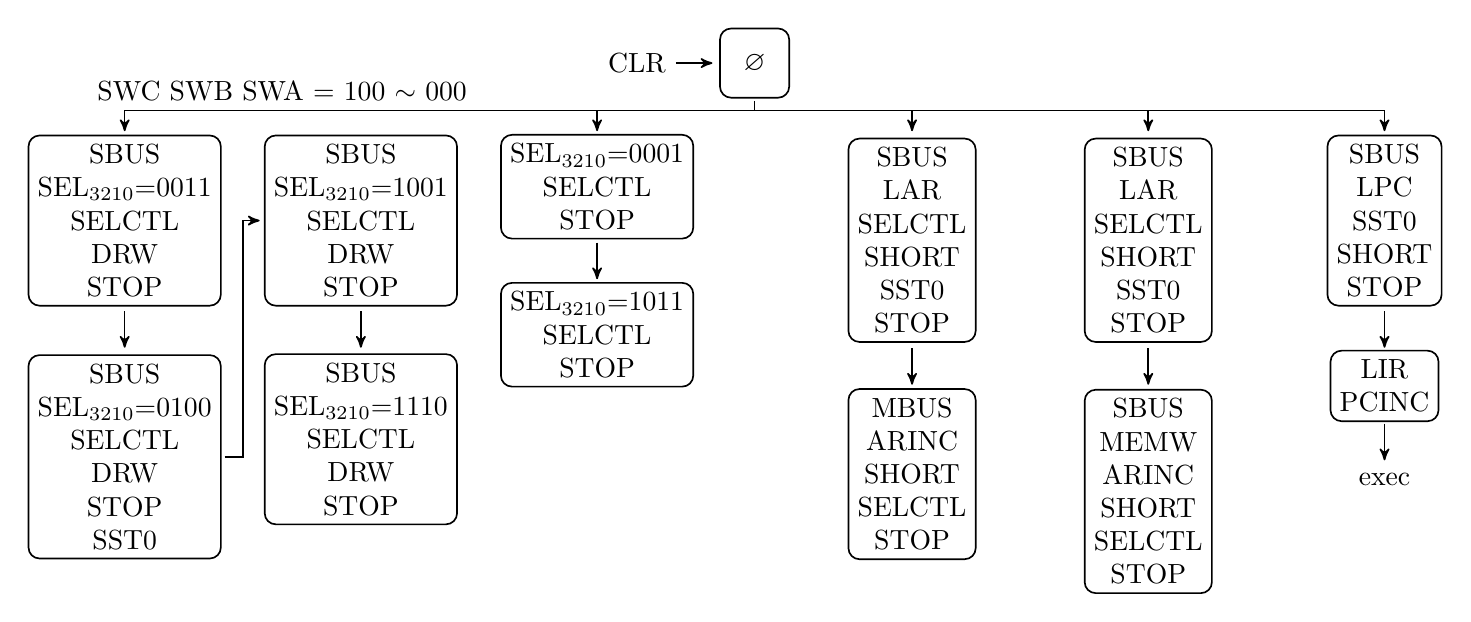
\begin{tikzpicture}[->,>=stealth',shorten >=1pt,auto,node distance=2.8cm,semithick]
    \tikzstyle{every state}=[shape=rectangle, rounded corners]
	\node[left] (clr) at (-1, 0) {CLR}; 
	\draw [->] (-1, 0) -- (-0.5,0);
	\node[state] (A) at (0, 0) {$\varnothing$};
	\node[state, align=center] (readra) at ( -8, -2) {SBUS\\ $\text{SEL}_{3210}$=0011\\ SELCTL\\ DRW\\ STOP};
	
	\node[state, align=center] (readrb) at ( -5, -2) {SBUS\\ $\text{SEL}_{3210}$=1001\\ SELCTL\\ DRW\\ STOP};

	\node[state, align=center] (readrc) at ( -8, -5) {SBUS\\ $\text{SEL}_{3210}$=0100\\ SELCTL\\ DRW\\ STOP\\ SST0};

	\node[state, align=center] (readrd) at ( -5, -4.777 ) {SBUS\\ $\text{SEL}_{3210}$=1110\\ SELCTL\\ DRW\\ STOP};
	
	\node[state, align=center] (readrd) at ( -2, -1.57 ) {$\text{SEL}_{3210}$=0001\\ SELCTL\\ STOP};
	\node[state, align=center] (readrd) at ( -2, -3.45 ) {$\text{SEL}_{3210}$=1011\\ SELCTL\\ STOP};

	\node[state, align=center] (readrd) at ( 2, -2.25 ) {SBUS\\ LAR\\ SELCTL\\ SHORT \\ SST0\\ STOP};
	\node[state, align=center] (readrd) at ( 2, -5.22 ) {MBUS\\ ARINC\\ SHORT\\ SELCTL\\ STOP};

	\node[state, align=center] (readrd) at ( 5, -2.25 ) {SBUS\\ LAR\\ SELCTL\\ SHORT \\ SST0\\ STOP};
	\node[state, align=center] (readrd) at ( 5, -5.44 ) {SBUS\\ MEMW\\ ARINC\\ SHORT\\ SELCTL\\ STOP};

	\node[state, align=center] (readrd) at ( 8, -2 ) {SBUS\\ LPC\\ SST0\\ SHORT\\ STOP};
	\node[state, align=center] (readrd) at ( 8, -4.10 ) {LIR \\ PCINC};
	%\path (A) edge[bend left] (B)
	\draw [->] (0, -0.48) -- (0, -0.6) -- (-8, -0.6) -- (-8, -0.9);
	\draw [->] (-8, -3.15) -- (-8, -3.65);
	\draw [->] (-6.73, -5) -- (-6.5, -5) -- (-6.5, -2) -- (-6.25, -2);
	\draw [->] (-5, -3.15) -- (-5, -3.65);

	\draw [->] (-2, -0.6) -- (-2, -0.9);
	\draw [->] (-2, -2.28) -- (-2, -2.78);

	\draw [->] (0, -0.6) -- (2, -0.6)-- (2, -0.9);
	\draw [->] (2, -3.62) -- (2, -4.12);
	
	\draw [->] (2, -0.6) -- (5, -0.6) -- (5, -0.9);
	\draw [->] (5, -3.62) -- (5, -4.12);
	
	\draw [->] (5, -0.6) -- (8, -0.6) -- (8, -0.9);

	\draw [->] (8, -3.15) -- (8, -3.65);
	\draw [->] (8, -4.58) -- (8, -5.08) node [below] {exec};

	\node [above] at (-6, -0.6) {SWC SWB SWA = 100 $\sim$ 000};
    \end{tikzpicture}
\end{figure}
\subsubsection{翻译成硬连线信号}
SBUS $\leftarrow$
\begin{enumerate}[\indent\indent]
	\item $(\text{W1} + \text{W2}) \cdot \text{SWC} \cdot \overline{\text{SWB}} \cdot \overline{\text{SWA}}$+
	\item $\text{W1} \cdot \overline{\text{SWC}} \cdot \text{SWB} \cdot \overline{\text{SWA}} \cdot \overline {\text{ST0}}$+
	\item $\text{W1} \cdot \overline{\text{SWC}} \cdot\overline{\text{SWB}}\cdot  \text{SWA}$+
​	\item $\text{W1} \cdot \overline{\text{SWC}} \cdot\overline{\text{SWB}}\cdot \overline{\text{SWA}}\cdot \overline{\text{ST0}} $
\end{enumerate}

MBUS $\leftarrow$
\begin{enumerate}[\indent\indent]
	\item $\text{W1} \cdot \overline{\text{SWC}} \cdot \text{SWB} \cdot \overline{\text{SWA}} \cdot \text{ST0}$+
	\item $\text{W2} \cdot \overline{\text{IR7}} \cdot \text{IR6} \cdot \overline{\text{IR5}} \cdot \text{IR4} \cdot \overline{\text{SWC}} \cdot\overline{\text{SWB}}\cdot \overline{\text{SWA}}$
\end{enumerate}

ABUS $\leftarrow$
\begin{enumerate}[\indent\indent]
	\item $\overline{\text{SWC}} \cdot\overline{\text{SWB}}\cdot \overline{\text{SWA}} \cdot \overline{\text{IR7}} \cdot \overline{\text{IR6}} \cdot \overline{\text{IR5}} \cdot \text{IR4} \cdot \text{W1}$+
	\item $\overline{\text{SWC}} \cdot\overline{\text{SWB}}\cdot \overline{\text{SWA}} \cdot \overline{\text{IR7}} \cdot \overline{\text{IR6}} \cdot \text{IR5} \cdot \overline{\text{IR4}} \cdot \text{W1}$+
	\item $\overline{\text{SWC}} \cdot\overline{\text{SWB}}\cdot \overline{\text{SWA}} \cdot \overline{\text{IR7}} \cdot \overline{\text{IR6}} \cdot \text{IR5} \cdot \text{IR4} \cdot \text{W1}$+
	\item $\overline{\text{SWC}} \cdot\overline{\text{SWB}}\cdot \overline{\text{SWA}} \cdot \overline{\text{IR7}} \cdot \text{IR6} \cdot \overline{\text{IR5}} \cdot \overline{\text{IR4}} \cdot \text{W1}$+
	\item $\overline{\text{SWC}} \cdot\overline{\text{SWB}}\cdot \overline{\text{SWA}} \cdot \overline{\text{IR7}} \cdot \text{IR6} \cdot \overline{\text{IR5}} \cdot \text{IR4} \cdot \text{W1}$+
	\item $\overline{\text{SWC}} \cdot\overline{\text{SWB}}\cdot \overline{\text{SWA}} \cdot \overline{\text{IR7}} \cdot \text{IR6} \cdot \text{IR5} \cdot \overline{\text{IR4}} \cdot (\text{W1} + \text{W2})$+
	\item $\overline{\text{SWC}} \cdot\overline{\text{SWB}}\cdot \overline{\text{SWA}} \cdot \text{IR7} \cdot \overline{\text{IR6}} \cdot \overline{\text{IR5}} \cdot \text{IR4} \cdot \text{W1}$+
	\item $\overline{\text{SWC}} \cdot\overline{\text{SWB}}\cdot \overline{\text{SWA}} \cdot \text{IR7} \cdot \overline{\text{IR6}} \cdot \text{IR5} \cdot \overline{\text{IR4}} \cdot \text{W1}$
\end{enumerate}

LAR $\leftarrow$
\begin{enumerate}[\indent\indent]
	\item $\text{W1} \cdot \overline{\text{SWC}} \cdot \text{SWB} \cdot \overline{\text{SWA}} \cdot \overline{\text{ST0}}$+
	\item $\text{W1} \cdot \overline{\text{SWC}} \cdot \overline{\text{SWB}} \cdot \text{SWA} \cdot \overline{\text{ST0}}$+
	\item $\overline{\text{SWC}} \cdot\overline{\text{SWB}}\cdot \overline{\text{SWA}} \cdot \overline{\text{IR7}} \cdot \text{IR6} \cdot \overline{\text{IR5}} \cdot \text{IR4} \cdot \text{W1}$+
	\item $\overline{\text{SWC}} \cdot\overline{\text{SWB}}\cdot \overline{\text{SWA}} \cdot \overline{\text{IR7}} \cdot \text{IR6} \cdot \text{IR5} \cdot \overline{\text{IR4}} \cdot \text{W1}$
\end{enumerate}

SST0 $\leftarrow$
\begin{enumerate}[\indent\indent]
	\item $\text{W1} \cdot \overline{\text{SWC}} \cdot \text{SWB} \cdot \overline{\text{SWA}} \cdot \overline{\text{ST0}}$+
	\item $\text{W2} \cdot \text{SWC} \cdot \overline{\text{SWB}} \cdot \overline{\text{SWA}} \cdot \overline{\text{ST0}}$+
	\item $\text{W1} \cdot \overline{\text{SWC}} \cdot \overline{\text{SWB}} \cdot \text{SWA} \cdot \overline{\text{ST0}}$+
	\item $\text{W1} \cdot \overline{\text{SWC}} \cdot \overline{\text{SWB}} \cdot \overline{\text{SWA}} \cdot \overline{\text{ST0}}$
\end{enumerate}

SHORT $\leftarrow$
\begin{enumerate}[\indent\indent]
	\item $\text{W1} \cdot \overline{\text{SWC}} \cdot \text{SWB} \cdot \overline{\text{SWA}}$
	\item $\text{W1} \cdot \overline{\text{SWC}} \cdot \overline{\text{SWB}} \cdot \text{SWA}$
	\item $\text{W1} \cdot \overline{\text{SWC}} \cdot \overline{\text{SWB}} \cdot \overline{\text{SWA}} \cdot \overline{ST0}$+
	\item $\overline{\text{SWC}} \cdot\overline{\text{SWB}}\cdot \overline{\text{SWA}} \cdot \overline{\text{IR7}} \cdot \overline{\text{IR6}} \cdot \overline{\text{IR5}} \cdot \overline{\text{IR4}} \cdot \text{W1}$+
	\item $\overline{\text{SWC}} \cdot\overline{\text{SWB}}\cdot \overline{\text{SWA}} \cdot \overline{\text{IR7}} \cdot \overline{\text{IR6}} \cdot \overline{\text{IR5}} \cdot \text{IR4} \cdot \text{W1}$+
	\item $\overline{\text{SWC}} \cdot\overline{\text{SWB}}\cdot \overline{\text{SWA}} \cdot \overline{\text{IR7}} \cdot \overline{\text{IR6}} \cdot \text{IR5} \cdot \overline{\text{IR4}} \cdot \text{W1}$+
	\item $\overline{\text{SWC}} \cdot\overline{\text{SWB}}\cdot \overline{\text{SWA}} \cdot \overline{\text{IR7}} \cdot \overline{\text{IR6}} \cdot \text{IR5} \cdot \text{IR4} \cdot \text{W1}$+
	\item $\overline{\text{SWC}} \cdot\overline{\text{SWB}}\cdot \overline{\text{SWA}} \cdot \overline{\text{IR7}} \cdot \text{IR6} \cdot \overline{\text{IR5}} \cdot \overline{\text{IR4}} \cdot \text{W1}$+
	\item $\overline{\text{SWC}} \cdot\overline{\text{SWB}}\cdot \overline{\text{SWA}} \cdot \overline{\text{IR7}} \cdot \text{IR6} \cdot \text{IR5} \cdot \text{IR4} \cdot \text{W1} \cdot \overline{C}$+
	\item $\overline{\text{SWC}} \cdot\overline{\text{SWB}}\cdot \overline{\text{SWA}} \cdot \text{IR7} \cdot \overline{\text{IR6}} \cdot \overline{\text{IR5}} \cdot \overline{\text{IR4}} \cdot \text{W1} \cdot \overline{Z}$
\end{enumerate}


ARINC $\leftarrow$
\begin{enumerate}[\indent\indent]
	\item $\text{W1} \cdot \overline{\text{SWC}} \cdot \text{SWB} \cdot \overline{\text{SWA}} \cdot \text{ST0}$+
	\item $\text{W1} \cdot \overline{\text{SWC}} \cdot \overline{\text{SWB}} \cdot \text{SWA} \cdot \text{ST0}$
\end{enumerate}

MEMW $\leftarrow$
\begin{enumerate}[\indent\indent]
	\item $\text{W1} \cdot \overline{\text{SWC}} \cdot \overline{\text{SWB}} \cdot \text{SWA} \cdot \text{ST0}$+
	\item $\overline{\text{SWC}} \cdot\overline{\text{SWB}}\cdot \overline{\text{SWA}} \cdot \overline{\text{IR7}} \cdot \text{IR6} \cdot \text{IR5} \cdot \overline{\text{IR4}} \cdot \text{W2}$
\end{enumerate}

LIR $\leftarrow$
\begin{enumerate}[\indent\indent]
	\item $\overline{\text{SWC}} \cdot\overline{\text{SWB}}\cdot \overline{\text{SWA}} \cdot \overline{\text{IR7}} \cdot \overline{\text{IR6}} \cdot \overline{\text{IR5}} \cdot \overline{\text{IR4}} \cdot \text{W1}$+
	\item $\overline{\text{SWC}} \cdot\overline{\text{SWB}}\cdot \overline{\text{SWA}} \cdot \overline{\text{IR7}} \cdot \overline{\text{IR6}} \cdot \overline{\text{IR5}} \cdot \text{IR4} \cdot \text{W1}$+
	\item $\overline{\text{SWC}} \cdot\overline{\text{SWB}}\cdot \overline{\text{SWA}} \cdot \overline{\text{IR7}} \cdot \overline{\text{IR6}} \cdot \text{IR5} \cdot \overline{\text{IR4}} \cdot \text{W1}$+
	\item $\overline{\text{SWC}} \cdot\overline{\text{SWB}}\cdot \overline{\text{SWA}} \cdot \overline{\text{IR7}} \cdot \overline{\text{IR6}} \cdot \text{IR5} \cdot \text{IR4} \cdot \text{W1}$+
	\item $\overline{\text{SWC}} \cdot\overline{\text{SWB}}\cdot \overline{\text{SWA}} \cdot \overline{\text{IR7}} \cdot \text{IR6} \cdot \overline{\text{IR5}} \cdot \overline{\text{IR4}} \cdot \text{W1}$+
	\item $\overline{\text{SWC}} \cdot\overline{\text{SWB}}\cdot \overline{\text{SWA}} \cdot \overline{\text{IR7}} \cdot \text{IR6} \cdot \text{IR5} \cdot \text{IR4} \cdot \text{W1} \cdot \overline{C}$+
	\item $\overline{\text{SWC}} \cdot\overline{\text{SWB}}\cdot \overline{\text{SWA}} \cdot \text{IR7} \cdot \overline{\text{IR6}} \cdot \overline{\text{IR5}} \cdot \overline{\text{IR4}} \cdot \text{W1} \cdot \overline{Z}$+
	\item $\overline{\text{SWC}} \cdot\overline{\text{SWB}}\cdot \overline{\text{SWA}} \cdot \overline{\text{IR7}} \cdot \text{IR6} \cdot \text{IR5} \cdot \text{IR4} \cdot \text{W2} \cdot C$+
	\item $\overline{\text{SWC}} \cdot\overline{\text{SWB}}\cdot \overline{\text{SWA}} \cdot \text{IR7} \cdot \overline{\text{IR6}} \cdot \overline{\text{IR5}} \cdot \overline{\text{IR4}} \cdot \text{W2} \cdot Z$+
	\item $\text{W2} \cdot \overline{\text{IR7}} \cdot \text{IR6} \cdot \overline{\text{IR5}} \cdot \text{IR4} \cdot \overline{\text{SWC}} \cdot\overline{\text{SWB}}\cdot \overline{\text{SWA}}$+
	\item $\overline{\text{SWC}} \cdot\overline{\text{SWB}}\cdot \overline{\text{SWA}} \cdot \overline{\text{IR7}} \cdot \text{IR6} \cdot \text{IR5} \cdot \overline{\text{IR4}} \cdot \text{W2}$+
	\item $\overline{\text{SWC}}\cdot\overline{\text{SWB}}\cdot\overline{\text{SWA}}\cdot\overline{\text{ST0}}\cdot\text{W1}$
\end{enumerate}

CIN $\leftarrow$
\begin{enumerate}[\indent\indent]
	\item $\overline{\text{SWC}} \cdot\overline{\text{SWB}}\cdot \overline{\text{SWA}} \cdot \overline{\text{IR7}} \cdot \overline{\text{IR6}} \cdot \overline{\text{IR5}} \cdot \overline{\text{IR4}} \cdot \text{W1}$
\end{enumerate}

M $\leftarrow$
\begin{enumerate}[\indent\indent]
	\item $\overline{\text{SWC}} \cdot\overline{\text{SWB}}\cdot \overline{\text{SWA}} \cdot \overline{\text{IR7}} \cdot \overline{\text{IR6}} \cdot \text{IR5} \cdot \text{IR4} \cdot \text{W2}$+
	\item $\overline{\text{SWC}} \cdot\overline{\text{SWB}}\cdot \overline{\text{SWA}} \cdot \overline{\text{IR7}} \cdot \text{IR6} \cdot \overline{\text{IR5}} \cdot \text{IR4} \cdot \text{W2}$+
	\item $\overline{\text{SWC}} \cdot\overline{\text{SWB}}\cdot \overline{\text{SWA}} \cdot \overline{\text{IR7}} \cdot \text{IR6} \cdot \text{IR5} \cdot \overline{\text{IR4}} \cdot (\text{W2} + \text{W3})$+
	\item $\overline{\text{SWC}} \cdot\overline{\text{SWB}}\cdot \overline{\text{SWA}} \cdot \text{IR7} \cdot \overline{\text{IR6}} \cdot \overline{\text{IR5}} \cdot \text{IR4} \cdot \text{W2}$+
	\item $\overline{\text{SWC}} \cdot\overline{\text{SWB}}\cdot \overline{\text{SWA}} \cdot \text{IR7} \cdot \overline{\text{IR6}} \cdot \text{IR5} \cdot \overline{\text{IR4}} \cdot \text{W2}$
\end{enumerate}

SEL0$\leftarrow$
\begin{enumerate}[\indent\indent]
	\item$\text{SWC}\cdot\overline{\text{SWB}}\cdot\overline{\text{SWA}}\cdot\text{W1}$
\end{enumerate}

SEL1$\leftarrow$
\begin{enumerate}[\indent\indent]
	\item$\text{SWC}\cdot\overline{\text{SWB}}\cdot\overline{\text{SWA}}\cdot\text{W2}\cdot\text{ST0}$+
	\item$\text{SWC}\cdot\overline{\text{SWB}}\cdot\overline{\text{SWA}}\cdot\text{W1}\cdot\overline{\text{ST0}}$
\end{enumerate}

SEL2$\leftarrow$
\begin{enumerate}[\indent\indent]
	\item$\text{SWC}\cdot\overline{\text{SWB}}\cdot\overline{\text{SWA}}\cdot\text{W2}$
\end{enumerate}

SEL3$\leftarrow$
\begin{enumerate}[\indent\indent]
	\item$\text{SWC}\cdot\overline{\text{SWB}}\cdot\overline{\text{SWA}}\cdot\text{W1}\cdot\text{ST0}$+
	\item$\text{SWC}\cdot\overline{\text{SWB}}\cdot\overline{\text{SWA}}\cdot\text{W2}\cdot\overline{\text{ST0}}$
\end{enumerate}
STOP$\leftarrow$
\begin{enumerate}[\indent\indent]
	\item$\text{SWA}+\text{SWB}+\text{SWC}$+
	\item$\overline{\text{SWC}}\cdot\overline{\text{SWB}}\cdot\overline{\text{SWA}}\cdot {\text{IR7}} \cdot {\text{IR6}}\cdot {\text{IR5}}\cdot \overline{\text{IR4}} \cdot \text{ST0}\cdot \text{W2}$
\end{enumerate}
SELCTL$\leftarrow$
\begin{enumerate}[\indent\indent]
	\item$\overline{\text{SWA}}+\overline{\text{SWB}}+\overline{\text{SWC}}$
\end{enumerate}
DRW$\leftarrow$
\begin{enumerate}[\indent\indent]
	\item$\text{SWC}\cdot\overline{\text{SWB}}\cdot\overline{\text{SWA}}$+
	\item$\overline{\text{SWC}}\cdot\overline{\text{SWB}}\cdot\overline{\text{SWA}}\cdot\text{ST0}\cdot\overline{\text{IR7}}\cdot\overline{\text{IR6}}\cdot\overline{\text{IR5}}\cdot\text{IR4}\cdot\text{W2}$+
	\item$\overline{\text{SWC}}\cdot\overline{\text{SWB}}\cdot\overline{\text{SWA}}\cdot\text{ST0}\cdot\overline{\text{IR7}}\cdot\overline{\text{IR6}}\cdot{\text{IR5}}\cdot\overline{\text{IR4}}\cdot\text{W2}$+
	\item$\overline{\text{SWC}}\cdot\overline{\text{SWB}}\cdot\overline{\text{SWA}}\cdot\text{ST0}\cdot\overline{\text{IR7}}\cdot\overline{\text{IR6}}\cdot\text{IR5}\cdot\text{IR4}\cdot\text{W2}$+
	\item$\overline{\text{SWC}}\cdot\overline{\text{SWB}}\cdot\overline{\text{SWA}}\cdot\text{ST0}\cdot\overline{\text{IR7}}\cdot{\text{IR6}}\cdot\overline{\text{IR5}}\cdot\overline{\text{IR4}}\cdot\text{W2}$+
	\item$\overline{\text{SWC}}\cdot\overline{\text{SWB}}\cdot\overline{\text{SWA}}\cdot\text{ST0}\cdot\overline{\text{IR7}}\cdot{\text{IR6}}\cdot\overline{\text{IR5}}\cdot{\text{IR4}}\cdot\text{W3}$
\end{enumerate}
PCADD$\leftarrow$
\begin{enumerate}[\indent\indent]
	\item$\overline{\text{SWC}}\cdot\overline{\text{SWB}}\cdot\overline{\text{SWA}}\cdot\text{ST0}\cdot\overline{\text{IR7}}\cdot{\text{IR6}}\cdot{\text{IR5}}\cdot{\text{IR4}}\cdot\text{C}\cdot\text{W2}$+
	\item$\overline{\text{SWC}}\cdot\overline{\text{SWB}}\cdot\overline{\text{SWA}}\cdot\text{ST0}\cdot{\text{IR7}}\cdot\overline{\text{IR6}}\cdot\overline{\text{IR5}}\cdot\overline{\text{IR4}}\cdot\text{Z}\cdot\text{W2}$
\end{enumerate}
PCINC $\leftarrow$
\begin{enumerate}[\indent\indent]
	\item $\overline{\text{SWC}} \cdot\overline{\text{SWB}}\cdot \overline{\text{SWA}} \cdot \overline{\text{IR7}} \cdot \overline{\text{IR6}} \cdot \overline{\text{IR5}} \cdot \overline{\text{IR4}} \cdot \text{W1}$+
	\item $\overline{\text{SWC}} \cdot\overline{\text{SWB}}\cdot \overline{\text{SWA}} \cdot \overline{\text{IR7}} \cdot \overline{\text{IR6}} \cdot \overline{\text{IR5}} \cdot \text{IR4} \cdot \text{W1}$+
	\item $\overline{\text{SWC}} \cdot\overline{\text{SWB}}\cdot \overline{\text{SWA}} \cdot \overline{\text{IR7}} \cdot \overline{\text{IR6}} \cdot \text{IR5} \cdot \overline{\text{IR4}} \cdot \text{W1}$+
	\item $\overline{\text{SWC}} \cdot\overline{\text{SWB}}\cdot \overline{\text{SWA}} \cdot \overline{\text{IR7}} \cdot \overline{\text{IR6}} \cdot \text{IR5} \cdot \text{IR4} \cdot \text{W1}$+
	\item $\overline{\text{SWC}} \cdot\overline{\text{SWB}}\cdot \overline{\text{SWA}} \cdot \overline{\text{IR7}} \cdot \text{IR6} \cdot \overline{\text{IR5}} \cdot \overline{\text{IR4}} \cdot \text{W1}$+
	\item $\overline{\text{SWC}} \cdot\overline{\text{SWB}}\cdot \overline{\text{SWA}} \cdot \overline{\text{IR7}} \cdot \text{IR6} \cdot \text{IR5} \cdot \text{IR4} \cdot \text{W1} \cdot \overline{C}$+
	\item $\overline{\text{SWC}} \cdot\overline{\text{SWB}}\cdot \overline{\text{SWA}} \cdot \text{IR7} \cdot \overline{\text{IR6}} \cdot \overline{\text{IR5}} \cdot \overline{\text{IR4}} \cdot \text{W1} \cdot \overline{Z}$+
	\item $\overline{\text{SWC}} \cdot\overline{\text{SWB}}\cdot \overline{\text{SWA}} \cdot \overline{\text{IR7}} \cdot \text{IR6} \cdot \text{IR5} \cdot \text{IR4} \cdot \text{W2} \cdot C$+
	\item $\overline{\text{SWC}} \cdot\overline{\text{SWB}}\cdot \overline{\text{SWA}} \cdot \text{IR7} \cdot \overline{\text{IR6}} \cdot \overline{\text{IR5}} \cdot \overline{\text{IR4}} \cdot \text{W2} \cdot Z$+
	\item $\text{W2} \cdot \overline{\text{IR7}} \cdot \text{IR6} \cdot \overline{\text{IR5}} \cdot \text{IR4} \cdot \overline{\text{SWC}} \cdot\overline{\text{SWB}}\cdot \overline{\text{SWA}}$+
	\item $\overline{\text{SWC}} \cdot\overline{\text{SWB}}\cdot \overline{\text{SWA}} \cdot \overline{\text{IR7}} \cdot \text{IR6} \cdot \text{IR5} \cdot \overline{\text{IR4}} \cdot \text{W2}$+
	\item $\overline{\text{SWC}}\cdot\overline{\text{SWB}}\cdot\overline{\text{SWA}}\cdot\overline{\text{ST0}}\cdot\text{W1}$
\end{enumerate}
LPC$\leftarrow$
\begin{enumerate}[\indent\indent]
	\item$\overline{\text{SWC}}\cdot\overline{\text{SWB}}\cdot\overline{\text{SWA}}\cdot\overline{\text{ST0}}\cdot\text{W1}$
\end{enumerate}
LDC$\leftarrow$
\begin{enumerate}[\indent\indent]
	\item$\overline{\text{SWC}}\cdot\overline{\text{SWB}}\cdot\overline{\text{SWA}}\cdot\text{ST0}\cdot\overline{\text{IR7}}\cdot\overline{\text{IR6}}\cdot\overline{\text{IR5}}\cdot\text{IR4}\cdot\text{W1}$+
	\item$\overline{\text{SWC}}\cdot\overline{\text{SWB}}\cdot\overline{\text{SWA}}\cdot\text{ST0}\cdot\overline{\text{IR7}}\cdot\overline{\text{IR6}}\cdot{\text{IR5}}\cdot\overline{\text{IR4}}\cdot\text{W1}$+
	\item$\overline{\text{SWC}}\cdot\overline{\text{SWB}}\cdot\overline{\text{SWA}}\cdot\text{ST0}\cdot\overline{\text{IR7}}\cdot\overline{\text{IR6}}\cdot\text{IR5}\cdot\text{IR4}\cdot\text{W1}$+
	\item$\overline{\text{SWC}}\cdot\overline{\text{SWB}}\cdot\overline{\text{SWA}}\cdot\text{ST0}\cdot\overline{\text{IR7}}\cdot{\text{IR6}}\cdot\overline{\text{IR5}}\cdot\overline{\text{IR4}}\cdot\text{W1}$
\end{enumerate}
LDZ$\leftarrow$
\begin{enumerate}[\indent\indent]
	\item$\overline{\text{SWC}}\cdot\overline{\text{SWB}}\cdot\overline{\text{SWA}}\cdot\text{ST0}\cdot\overline{\text{IR7}}\cdot\overline{\text{IR6}}\cdot\overline{\text{IR5}}\cdot\text{IR4}\cdot\text{W1}$+
	\item$\overline{\text{SWC}}\cdot\overline{\text{SWB}}\cdot\overline{\text{SWA}}\cdot\text{ST0}\cdot\overline{\text{IR7}}\cdot\overline{\text{IR6}}\cdot{\text{IR5}}\cdot\overline{\text{IR4}}\cdot\text{W1}$+
	\item$\overline{\text{SWC}}\cdot\overline{\text{SWB}}\cdot\overline{\text{SWA}}\cdot\text{ST0}\cdot\overline{\text{IR7}}\cdot\overline{\text{IR6}}\cdot\text{IR5}\cdot\text{IR4}\cdot\text{W1}$+
	\item$\overline{\text{SWC}}\cdot\overline{\text{SWB}}\cdot\overline{\text{SWA}}\cdot\text{ST0}\cdot\overline{\text{IR7}}\cdot{\text{IR6}}\cdot\overline{\text{IR5}}\cdot\overline{\text{IR4}}\cdot\text{W1}$
\end{enumerate}
\subsubsection{翻译成多分支程序}
{\firacode
\begin{lstlisting}[language={VHDL}]
library IEEE;
use IEEE.std_logic_1164.all;
use IEEE.std_logic_unsigned.all;
entity CPU is
	port (
		CLR,C,Z,T3,W1,W2,W3: in std_logic;
		IRH:in std_logic_vector(3 downto 0);
		SWCBA:in std_logic_vector(2 downto 0);
		SELCTL,ABUS,M,SEL1,SEL0,SEL2,SEL3,DRW,SBUS,LIR,MBUS,MEMW,LAR,ARINC,LPC,
		PCINC,PCADD,CIN,LONG,SHORT,STOP,LDC,LDZ: out std_logic;
		S:out std_logic_vector(3 downto 0);
		CP1,CP2,CP3:out std_logic;	
		QD:in std_logic	
	);
end CPU;

architecture arc of CPU is
signal ST0,ST0_1,ST0_2,STOP_1,STOP_2: std_logic;
begin
	
	CP1 <= '1';
	CP2 <= '1';
	CP3 <= QD;

	with SWCBA select
		STOP <= '0'						when "000",
				STOP_1 or STOP_2 		when others;
	ST0 <= ST0_1;

	process (CLR, T3)
	begin
		-- 任何时候按下CLR, 都会返回
		if (CLR = '0') then
			ST0_1	<= '0';
			STOP_1	<= '1';
		-- 如果到节拍电位T3下降沿,ST0_1 |= ST0_2
		elsif (T3'event and T3 = '0') then
			if (ST0_2 = '1') then
				ST0_1 <= '1';
			end if;
		end if;
	end process;

	process (SWCBA, IRH, W1, W2, W3, ST0, C, Z)
	begin
		-- 初始化 和 状态参数
		SHORT <= '0';
		LONG <= '0';
		-- 设置STOP
		STOP_2 <= '1';
		-- 设置ST0标志
		ST0_2 <= '0';
		-- ALU
		ABUS <= '0';
		M <= '0';
		CIN <= '0';
		S <= "0000";
		ARINC <= '0';
		-- 保存Z标志
		LDZ <= '0';
		-- 保存C标志
		LDC <= '0';
		SBUS <= '0';
		MBUS <= '0';
		-- 控制台操作标志
		SELCTL <= '0';
		-- RD1~RD0
		SEL3 <= '0';
		SEL2 <= '0';
		-- RS1~RS0
		SEL1 <= '0';
		SEL0 <= '0';
		-- 送指令寄存器标志
		LIR <= '0';
		-- 送地址寄存器标志
		LAR <= '0';
		-- 送程序计数器标志
		LPC <= '0';
		-- (~R)/W
		MEMW <= '0';
		DRW <= '0';
		-- 程序计数器自增标志
		PCINC <= '0';		
		-- 程序计数器增量标志
		PCADD <= '0';
		case SWCBA is
			when "000" =>  --执行程序
				case ST0 is
					when '0' =>
						-- load pc
						LPC <= W1;
						SBUS <= W1;
						ST0_2 <= W1;
						SHORT <= W1;
						STOP_2 <= '0';
					when '1' =>
				case IRH is
					when "0000" =>  -- NOP
						-- 设定PC
						LIR <= W1;
						PCINC <= W1;
						-- 短周期
						SHORT <= W1;
					when "0001" =>  --ADD ()
						-- 设定PC
						LIR <= W1;
						PCINC <= W1;
						-- 短周期
						SHORT <= W1;
						-- ABUS = W1
						ABUS <= W1;
						CIN <= W1;
						-- 选择加法
						-- `选择算术运算,传送B`
						-- M已经被初始化为0
						S <= "1001";
						-- 加法操作
						DRW <= W1;
						LDZ <= W1;
						LDC <= W1;
					when "0010" =>  -- SUB ()
						-- 设定PC
						LIR <= W1;
						PCINC <= W1;
						-- 短周期
						SHORT <= W1;
						-- 选择算术运算, 选择减法
						-- M已经被初始化为0
						S <= "0110";
						-- 减法操作
						ABUS <= W1;
						DRW <= W1;
						LDZ <= W1;
						LDC <= W1;
					when "0011" =>  -- AND ()
						-- 设定PC
						LIR <= W1;
						PCINC <= W1;
						-- 短周期
						SHORT <= W1;
						-- 选择逻辑运算, 与运算
						M <= W1;
						S <= "1011";
						ABUS <= W1;
						DRW <= W1;
						LDZ <= W1;
					when "0100" => -- INC ()
						-- 设定PC
						LIR <= W1;
						PCINC <= W1;
						-- 短周期
						SHORT <= W1;
						-- 选择算术运算, 与运算
						-- M已经被初始化为0
						S <= "0000";
						ABUS <= W1;
						DRW <= W1;
						LDZ <= W1;
						LDC <= W1;
					when "0101" =>  -- LD
						-- `选择算术运算,传送B`
						M <= W1;
						S <= "1010";
						ABUS <= W1;
						LAR <= W1;
						-- 设定PC
						LIR <= W2;
						PCINC <= W2;
						MBUS <= W2;
						DRW <= W2;
					when "0110" =>  -- ST
						-- 设定...
						M <= W1 or W2;
						if(W1='1')then
							S<="1111";
						else
							S<="1010";
						end if;
						ABUS <= W1 or W2;
						LAR <= W1;
						MEMW <= W2;
						-- 设定PC
						LIR <= W2;
						PCINC <= W2;							
					when "0111" =>  -- JC
						-- 设定PC
						LIR <= (W1 and (not C)) or (W2 and C);
						PCINC <= (W1 and (not C)) or (W2 and C);
						PCADD <= C and W1;
						SHORT <= W1 and (not C);
					when "1000" =>  -- JZ
						-- 设定PC
						LIR <= (W1 and (not Z)) or (W2 and Z);
						PCINC <= (W1 and (not Z)) or (W2 and Z);
						PCADD <= Z and W1;
						SHORT <= W1 and (not Z);
					when "1001" =>  -- JMP
						-- 设定算术运算
						M <= W1;
						S <= "1111";
						ABUS <= W1;
						LPC <= W1;
						-- 设定PC
						LIR <= W2;
						PCINC <= W2;
					when "1010" =>  -- OUT
						-- 设定PC
						LIR <= W1;
						PCINC <= W1;
						-- 短周期
						SHORT <= W1;
						-- 设定算术运算
						M <= W1;
						S <= "1010";
						ABUS <= W1;
					when "1011" =>  -- SSP  
						SEL3<='1';
						M <= W1 or W2;
						if (W1 = '1') then
							S <= "1000";
						elsif (W2 = '1') then
							-- or S <= "1111"
							S <= "1010";
						end if;
						ABUS <= W1 or W2;
						LAR <= W1;
						MEMW <= W2;
						-- 设定PC
						LIR <= W2;
						PCINC <= W2;
					when "1100" =>  -- PUSH
						M <= W1 or W2;
						CIN <= W3;
						if (W1 = '1') then
							S <= "1111";
						elsif (W2 = '1') then
							S <= "1010";
						elsif (W3 = '1') then
							S <= "1111";
						end if;
						ABUS <= W1 or W2 or W3;
						LAR <= W1;
						MEMW <= W2;
						LONG <= W2;
						DRW <= W3;
						LIR <= W3;
						PCINC <= W3;
					when "1101" =>  -- MOV B->A
						-- 设定PC
						LIR <= W1;
						PCINC <= W1;
						-- 短周期
						SHORT <= W1;
						-- 选择逻辑运算, MOV 运算
						M <= W1;
						S <= "1010";
						ABUS <= W1;
						DRW <= W1;
						LDZ <= W1;
					when "1110" =>  -- STP
						STOP_2 <= W1;								
					when "1111" =>  -- LSP
						M <= W1;
						S <= "1000";
						ABUS <= W1;
						LAR <= W1;
						MBUS <= W2;
						DRW <= W2;
						-- 设定PC
						LIR <= W2;
						PCINC <= W2;				
					when others =>  -- 公操作
						-- 设定PC
						LIR <= W1;
						PCINC <= W1;
				end case;
					when others =>
						-- 不可能到这吧?
				end case;
			when "001" =>
			--	SEL0<=ST0;
				-- SBUS = (ST0=0 or ST0=1) and W1 
				SBUS <= W1;
				-- STOP = (ST0=0 or ST0=1) and W1
				STOP_2 <= W1;
				-- SHORT = (ST0=0 or ST0=1) and W1
				SHORT <= W1;
				-- SELCTL = (ST0=0 or ST0=1) and W1
				SELCTL <= W1;
				-- LAR = (ST0=0) and W1
				LAR <= W1 and (not ST0);
				-- LAR = (ST0=1) and W1
				ARINC <= W1 and ST0;
				-- MEMW = (ST0=1) and W1
				MEMW <= W1 and ST0;
				ST0_2 <= W1;
			when "010" =>
				-- SHORT = (ST0=0 or ST0=1) and W1
				SHORT<=W1;
				-- SELCTL = (ST0=0 or ST0=1) and W1
				SELCTL <= W1;
				-- STOP = (ST0=0 or ST0=1) and W1
				STOP_2<=W1;
				-- SBUS = (ST0=0) and W1
				SBUS<=W1 and (not ST0);
				-- LAR = (ST0=0) and W1
				LAR<=W1 and (not ST0);
				-- MBUS = (ST0=1) and W1
				MBUS<=W1 and ST0;
				-- ARINC = (ST0=1) and W1
				ARINC<=W1 and ST0;
				ST0_2<=W1;
			when "011" =>
				-- SELCTL = W1 or W2
				SELCTL <= '1';
				-- STOP = W1 or W2
				STOP_2 <= W1 or W2;
				-- SEL0 = W1 or W2
				SEL0<=W1 or W2;
				-- SEL1 = W2
				SEL1<=W2;
				-- SEL2 = 0
				-- SEL3 = W2
				SEL3<=W2;
			when "100" =>
				-- SELCTL = (ST0=0 or ST0=1) and (W1 or W2)
				SELCTL <= '1';
				-- SBUS = (ST0=0 or ST0=1) and (W1 or W2)
				SBUS <= W1 or W2;
				-- STOP = (ST0=0 or ST0=1) and (W1 or W2)
				STOP_2 <= W1 or W2;
				-- DRW = (ST0=0 or ST0=1) and (W1 or W2)
				DRW <= W1 or W2;
				-- SEL0 = (ST0=0 or ST0=1) and W1
				SEL0 <= W1;
				-- SEL1 = ((ST0=0) and W1) or ((ST0=1) and W2)
				SEL1 <= ((not ST0) and W1) or (ST0 and W2);
				-- SEL2 = (ST0=0 or ST0=1) and W2
				SEL2 <= W2;
				-- SEL3 = (ST0=1) and (W1 or W2) 
				SEL3 <= ST0 and (W1 or W2);
				ST0_2 <= W2;
			when others=>
		end case;
	end process;
end arc;
\end{lstlisting}
}

\section{调试过程中的问题及讨论}

\section{设计调试小结}
\end{document}